% !TEX root = ../notes_template.tex
\chapter{Vectors}\label{chp:vectors}

% \minitoc

\section{$n$-Vectors}
A collection of an ordered list of $n$ numbers is called an $n$-vector. We will use bold lower case alphabets to represent such vectors, and we will represent these as a column of numbers, which is referred to as a \textit{column vector}. We will look at \textit{row vectors} at a later stage. Consider the following example:
\[ \mf{x} = \bmxc x_1 \\ x_2 \\ \vdots \\x_n \emx \]

The elements of the $n$-vector $x_1, x_2, \ldots, x_n$ are called the \textit{components} of the vector $\mf{x}$; $x_i$ is the $i^{th}$ component of the vector $\mf{x}$. If these components are all real numbers, the set of all such $n$-vectors is the set $\mb{R}^n$.

\noindent \textbf{Where do we come across such $n$-vectors?} In many places, such as in physics, engineering, economics, medicine, etc. Any application where we deal with multiple pieces of information that can be represented as a list of numbers can be represented as an $n$-vector. When we deal with systems with multiple inputs, multiple output, or multiple states, we can represent these as $n$-vectors. We talk about the state of a system in a later chapter.

\section{Visualizing $n$-vectors}
The $n$-vectors can be visualized as points in $n$-dimensional space. For example, A 1-vector or just single real number or a \textit{scalar} can be thought of as a point on the real line. The 1-vector $x = 2.45$ is shown in Figure~\ref{fig:1-vector} is the red point. But we will find it useful to visualize a 1-vector as an arrow starting at the origin and ending at the point on the real line. The arrow is shown in blue in Figure~\ref{fig:1-vector}. 

\begin{figure}[b]
    \centering
    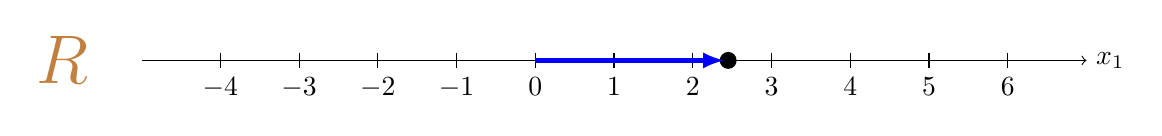
\begin{tikzpicture}
        \draw[->] (-5,0) -- (7,0) node[right] {$x_1$};
        \foreach \x in {,-4,-3,-2,0,-1,1,2,3,4,5,6}
            \draw (\x,0.1) -- (\x,-0.1) node[below] {$\x$};
        % Plot an example point and its corresponding arrow
        \draw[fill=black] (2.45,0) circle (0.1); % Smaller marker size
        \draw[-latex, ultra thick, blue] (0,0) -- (2.4,0); % Thicker arrow
        % Huge font for the label with brown color
        \node[font=\Huge, text=brown] at (-6, 0) {$\mathbb{R}$};
    \end{tikzpicture}
    \caption{The real line $\mb{R}$ contains the $1$-vectors.}
    \label{fig:1-vector}
\end{figure}

The elements of $\mb{R}^2$ are points on the plane, and we can visualize them as points in the plane. The 2-vectors $\mf{x} = \bmxc 2 \\ 3 \emx$ and $\mf{x} = \bmxc -3 \\ 1 \emx$ are shown in Figure~\ref{fig:2-vector}. A similar visualization is shown for $\mb{R}^3$ (Figure~\ref{fig:3-vector}), and for $\mb{R}^4$ and beyond you simply pretend that you can visualize things in your head like your instructor does.

\begin{figure}[t]
    \centering
    \begin{subfigure}[b]{0.45\textwidth}
        \centering
        \begin{tikzpicture}[scale=0.6]
            \draw[->, gray] (-5,0) -- (5,0) node[right] {$x_1$};
            \draw[->, gray] (0,-5) -- (0,5) node[above] {$x_2$};
            \foreach \x in {-4,-2,-1,2,4}
            \draw (\x,0.1) -- (\x,-0.1) node[below, gray] {$\x$};
            \foreach \y in {-4,-2,-1,2,4}
            \draw (0.1,\y) -- (-0.1,\y) node[left, gray] {$\y$};
            % Plot an example point and its corresponding arrow
            \draw[fill=black] (2,3) circle (0.1); % Marker for the point (2,3)
            \draw[-latex, ultra thick, blue] (0,0) --  (2,3) node[right, black] {$\mathbf{x} = \begin{bmatrix} 2 \\ 3 \end{bmatrix}$}; % Arrow with label
            
            \draw[fill=black] (-3,1) circle (0.1); % Marker for the point (-2,1)
            \draw[-latex, ultra thick, red] (0,0) --  (-3,1) node[left, black] {$\mathbf{y} = \begin{bmatrix} -3 \\ 1 \end{bmatrix}$}; % Arrow with label
            
            % Huge font for the label with brown color
            \node[font=\Huge, text=brown] at (-4, 4) {$\mathbb{R}^2$};
        \end{tikzpicture}
        \caption{The $\mathbb{R}^2$ plane contains the $2$-vectors.}
        \label{fig:2-vector}
    \end{subfigure}
    \begin{subfigure}[b]{0.45\textwidth}
        \centering
        \tdplotsetmaincoords{60}{120} % Set the view angle
        \begin{tikzpicture}[scale=0.7,tdplot_main_coords] % Set scale and use the main coordinates
            % Axis lines
            \draw[->, gray] (-5,0,0) -- (5,0,0) node[anchor=north east]{$x_1$};
            \draw[->, gray] (0,-5,0) -- (0,5,0) node[anchor=north west]{$x_2$};
            \draw[->, gray] (0,0,-5) -- (0,0,5) node[anchor=south]{$x_3$};
            \foreach \x in {-4,-2,,2,4}
                \draw (\x,0,0.1) -- (\x,0,-0.1) node[below, gray] {$\x$};
            \foreach \y in {-4,-2,,2,4}
                \draw (0.1,\y,0) -- (-0.1,\y,0) node[above right, gray] {$\y$};
            \foreach \z in {-4,-2,,2,4}
                \draw (0.1,0,\z) -- (-0.1,0,\z) node[above right, gray] {$\z$};
            % Points
            \draw[fill=blue] (1,2,3) circle (0.08);
            \draw[-latex, ultra thick, blue] (0,0,0) --  (1,2,3) node[above, black] {$\mathbf{x} = \bmx 1 \\ 2 \\ 1 \emx$}; 
            % Points
            \draw[fill=red] (2,-1,1) circle (0.08);
            \draw[-latex, ultra thick, red] (0,0,0) --  (2,-1,1) node[below left, black] {$\mathbf{y} = \bmx 2 \\ -1 \\ 1 \emx$}; 
             
            % Huge font for the label with brown color
            \node[font=\Huge, text=brown] at (2,-2,4.5) {$\mathbb{R}^3$};
        \end{tikzpicture}
        \caption{$\mb{R}^3$ contains the 3-vectors.}
        \label{fig:3-vector}
    \end{subfigure}
    \caption{The $\mb{R}^2$ and $\mb{R}^3$ sets.}
    \label{fig:combined}
\end{figure}

\section{Some Commonly Used $n$-vectors}
We will now define a some commonly used $n$-vectors that we will use in the course. 
\begin{itemize}
    \item \textbf{Zero vector:} The $n$-vector whose components are all zeros is called the \textit{zero vector}. $\mf{0} = \bmxc 0 \\ 0 \\ \vdots \\ 0\emx$
    \item \textbf{One vector:} The $n$-vector whose components are all ones is called the \textit{one vector}. $\mf{1} = \bmxc 1 \\ 1 \\ \vdots \\ 1\emx$
    \item \textbf{Unit vectors:} The $n$-vectors whose components are all zeros except for one component which is 1. These are called the \textit{standard basis vectors} and are denoted by $\mf{e}_1, \mf{e}_2, \ldots, \mf{e}_n$. The $n$-vector $\mf{e}_i$ has all components as zeros except for the $i^{th}$ component which is 1. For example, the unit vectors in $\mb{R}^2$ are:
    \[ \mf{e}_1 = \bmx 1 \\ 0\emx \quad \mf{e}_2 = \bmx 0 \\ 1 \emx  \]
\end{itemize}

\section{Operations on $n$-vectors}
There are many operations we can perform on $n$-vectors, but we will only focus on two operations for this:
\begin{itemize}
    \item \textbf{Scalar multiplication:} Given a scalar $c \in \mb{R}$ and an $n$-vector $\mf{x}$. The scalar multiplication operation produces another $n$-vector $c\mf{x}$ whose components are $cx_1, cx_2, \ldots, cx_n$. 
    \[ \mf{x} = \bmx 1 \\ 2\emx \longrightarrow 2 \mf{x} = \bmx  2\ct{1} \\ 2\ct{2} \emx = \bmx  2 \\ 8.2 \emx \]
    
    \item \textbf{Vector Addition:} Given two $n$-vectors $\mf{x}$ and $\mf{y}$, the vector addition operation, represented by $\mf{x} + \mf{y}$, producs another $n$-vector whose components are $x_1 + y_1, x_2 + y_2, \ldots, x_n + y_n$.
    \[ \mf{x} = \bmxc 1 \\ 3 \emx, \mf{y} = \bmxc 2 \\ 1 \emx \longrightarrow \mf{x} + \mf{y} = \bmxc 1 + 2 \\ 3 + 1 \emx = \bmxc 3 \\ 4 \emx \]
\end{itemize}
\begin{figure}[h]
    \centering
    \begin{tikzpicture}[scale=0.6]
        \draw[->, gray] (-5,0) -- (5,0) node[right] {$x_1$};
        \draw[->, gray] (0,-5) -- (0,5) node[above] {$x_2$};
        \foreach \x in {-4,-2,2,4}
        \draw (\x,0.1) -- (\x,-0.1) node[below, gray] {$\x$};
        \foreach \y in {-4,-2,2,4}
        \draw (0.1,\y) -- (-0.1,\y) node[left, gray] {$\y$};
        \draw[-latex, ultra thick, black] (0,0) --  (1,2) node[below right, black] {$\mf{x}$}; % Arrow with label
        \draw[-latex, thick, red] (0,0) --  (2,4) node[right, black] {$2\mf{x}$}; % Arrow with label
        \draw[-latex, thick, blue] (0,0) --  (-1.5,-3) node[left, black] {$-1.5\mf{x}$}; % Arrow with label
    \end{tikzpicture}
    \caption{Scalar multiplication of a vector.}
    \label{fig:scalar-mult}
\end{figure}

The geometric interpretation of these operations is shown in Figure~\ref{fig:scalar-mult} and Figure~\ref{fig:vec-add}. Scalar multiplication stretches or shrinks the vector without rotating the vector. When the scalar is positive the direction of the scaled vector is the same as the original vector, and when the scalar is negative the direction is opposite. When the scalar is zero, the scaled vector is the zero vector $\mf{0}$. 

Vector addition moves the vector to a new location without changing its direction. The vector $\mf{x} + \mf{y}$ is the vector that starts at the origin and ends at the point where the vector $\mf{x}$ ends and the vector $\mf{y}$ ends.

\begin{figure}[h]
    \centering
    \begin{tikzpicture}[scale=0.6]
        \draw[->, gray] (-5,0) -- (5,0) node[right] {$x_1$};
        \draw[->, gray] (0,-5) -- (0,5) node[above] {$x_2$};
        \foreach \x in {-4,-2,2,4}
        \draw (\x,0.1) -- (\x,-0.1) node[below, gray] {$\x$};
        \foreach \y in {-4,-2,2,4}
        \draw (0.1,\y) -- (-0.1,\y) node[left, gray] {$\y$};
        \draw[-latex, ultra thick, black] (0,0) --  (1,2) node[below right, black] {$\mf{x}$}; % Arrow with label
        \draw[-latex, thick, red] (0,0) --  (2,4) node[right, black] {$2\mf{x}$}; % Arrow with label
        \draw[-latex, thick, blue] (0,0) --  (-1.5,-3) node[left, black] {$-1.5\mf{x}$}; % Arrow with label
    \end{tikzpicture}
    \caption{Scalar multiplication of a vector.}
    \label{fig:scalar-mult}
\end{figure}


Vector addition moves the vector to a new location without changing its direction. The vector $\mf{x} + \mf{y}$ is the vector that starts at the origin and ends at the point where the vector $\mf{x}$ ends and the vector $\mf{y}$ ends.


gls example
\begin{itemize}
	% \item \glsxtrshort{gcd};
	\item \Gls{gcd}; \acrlong{gcd}; \acrshort{gcd}; \acrfull{gcd}
\end{itemize}

\section{Proof}
\begin{lemma}
\end{lemma}
\begin{claim}
\end{claim}
\begin{theorem}
\end{theorem}
\begin{example}
\end{example}
\begin{fact}
\end{fact}
\begin{remark}
\end{remark}
\begin{exercise}
	Prove A \iff B
\end{exercise}
\begin{solution}
By induction:
\end{solution}

\lipsum % dummy text - remove from real document

\section{Quantifier}
\lipsum % dummy text - remove from real document

\section{Graph}
\citetitle{babaiGraphIsomorphismQuasipolynomial2016}
\cite{babaiGraphIsomorphismQuasipolynomial2016}

\section{Number theory}
Figure example
\begin{figure}[!ht]
    \centering
    \includegraphics[width=1\linewidth]{./figure/elliptic_curves.pdf}
    \caption{Elliptic curves \cite{childsUniversalComputationQuantum2009} }
\end{figure}


\section{Algorithm}
% \begin{center}
% \begin{minipage}{.9\linewidth}
% algorithm2e
% https://www.overleaf.com/learn/latex/Algorithms#The_algorithm2e_package
\begin{algorithm}[H]
    \SetKwInOut{Input}{input}
    \SetKwInOut{Output}{output}
    \Input{Integer $N$ and parameter $1^t$}
    \Output{A decision as to whether $N$ is prime or composite}
    \BlankLine
    \For{ $i = 1,2, \ldots, t$} {
        $a\leftarrow \qty{1,\dots,N_1}$\;
        \If{$a^{N-1} \neq 1 \mod{N}$}
    {\Return "composite"}
    }
    \Return "prime"
    \caption{Primality testing - first attempt}
    \label{alg:miller_rabin}
\end{algorithm}
% \end{minipage}
% \end{center}